\documentclass[twoside]{book}

% Packages required by doxygen
\usepackage{fixltx2e}
\usepackage{calc}
\usepackage{doxygen}
\usepackage[export]{adjustbox} % also loads graphicx
\usepackage{graphicx}
\usepackage[utf8]{inputenc}
\usepackage{makeidx}
\usepackage{multicol}
\usepackage{multirow}
\PassOptionsToPackage{warn}{textcomp}
\usepackage{textcomp}
\usepackage[nointegrals]{wasysym}
\usepackage[table]{xcolor}

% Font selection
\usepackage[T1]{fontenc}
\usepackage[scaled=.90]{helvet}
\usepackage{courier}
\usepackage{amssymb}
\usepackage{sectsty}
\renewcommand{\familydefault}{\sfdefault}
\allsectionsfont{%
  \fontseries{bc}\selectfont%
  \color{darkgray}%
}
\renewcommand{\DoxyLabelFont}{%
  \fontseries{bc}\selectfont%
  \color{darkgray}%
}
\newcommand{\+}{\discretionary{\mbox{\scriptsize$\hookleftarrow$}}{}{}}

% Page & text layout
\usepackage{geometry}
\geometry{%
  a4paper,%
  top=2.5cm,%
  bottom=2.5cm,%
  left=2.5cm,%
  right=2.5cm%
}
\tolerance=750
\hfuzz=15pt
\hbadness=750
\setlength{\emergencystretch}{15pt}
\setlength{\parindent}{0cm}
\setlength{\parskip}{3ex plus 2ex minus 2ex}
\makeatletter
\renewcommand{\paragraph}{%
  \@startsection{paragraph}{4}{0ex}{-1.0ex}{1.0ex}{%
    \normalfont\normalsize\bfseries\SS@parafont%
  }%
}
\renewcommand{\subparagraph}{%
  \@startsection{subparagraph}{5}{0ex}{-1.0ex}{1.0ex}{%
    \normalfont\normalsize\bfseries\SS@subparafont%
  }%
}
\makeatother

% Headers & footers
\usepackage{fancyhdr}
\pagestyle{fancyplain}
\fancyhead[LE]{\fancyplain{}{\bfseries\thepage}}
\fancyhead[CE]{\fancyplain{}{}}
\fancyhead[RE]{\fancyplain{}{\bfseries\leftmark}}
\fancyhead[LO]{\fancyplain{}{\bfseries\rightmark}}
\fancyhead[CO]{\fancyplain{}{}}
\fancyhead[RO]{\fancyplain{}{\bfseries\thepage}}
\fancyfoot[LE]{\fancyplain{}{}}
\fancyfoot[CE]{\fancyplain{}{}}
\fancyfoot[RE]{\fancyplain{}{\bfseries\scriptsize Generated by Doxygen }}
\fancyfoot[LO]{\fancyplain{}{\bfseries\scriptsize Generated by Doxygen }}
\fancyfoot[CO]{\fancyplain{}{}}
\fancyfoot[RO]{\fancyplain{}{}}
\renewcommand{\footrulewidth}{0.4pt}
\renewcommand{\chaptermark}[1]{%
  \markboth{#1}{}%
}
\renewcommand{\sectionmark}[1]{%
  \markright{\thesection\ #1}%
}

% Indices & bibliography
\usepackage{natbib}
\usepackage[titles]{tocloft}
\setcounter{tocdepth}{3}
\setcounter{secnumdepth}{5}
\makeindex

% Hyperlinks (required, but should be loaded last)
\usepackage{ifpdf}
\ifpdf
  \usepackage[pdftex,pagebackref=true]{hyperref}
\else
  \usepackage[ps2pdf,pagebackref=true]{hyperref}
\fi
\hypersetup{%
  colorlinks=true,%
  linkcolor=blue,%
  citecolor=blue,%
  unicode%
}

% Custom commands
\newcommand{\clearemptydoublepage}{%
  \newpage{\pagestyle{empty}\cleardoublepage}%
}

\usepackage{caption}
\captionsetup{labelsep=space,justification=centering,font={bf},singlelinecheck=off,skip=4pt,position=top}

%===== C O N T E N T S =====

\begin{document}

% Titlepage & ToC
\hypersetup{pageanchor=false,
             bookmarksnumbered=true,
             pdfencoding=unicode
            }
\pagenumbering{alph}
\begin{titlepage}
\vspace*{7cm}
\begin{center}%
{\Large My Project }\\
\vspace*{1cm}
{\large Generated by Doxygen 1.8.13}\\
\end{center}
\end{titlepage}
\clearemptydoublepage
\pagenumbering{roman}
\tableofcontents
\clearemptydoublepage
\pagenumbering{arabic}
\hypersetup{pageanchor=true}

%--- Begin generated contents ---
\chapter{Hierarchical Index}
\section{Class Hierarchy}
This inheritance list is sorted roughly, but not completely, alphabetically\+:\begin{DoxyCompactList}
\item \contentsline{section}{Bank}{\pageref{classBank}}{}
\item \contentsline{section}{Cashier}{\pageref{classCashier}}{}
\item \contentsline{section}{Client}{\pageref{classClient}}{}
\item \contentsline{section}{Compare\+Event\+Priority}{\pageref{classCompareEventPriority}}{}
\item \contentsline{section}{Discrete\+Event\+Simulation}{\pageref{classDiscreteEventSimulation}}{}
\begin{DoxyCompactList}
\item \contentsline{section}{Simulation}{\pageref{classSimulation}}{}
\end{DoxyCompactList}
\item \contentsline{section}{Event}{\pageref{classEvent}}{}
\begin{DoxyCompactList}
\item \contentsline{section}{Arrival}{\pageref{classArrival}}{}
\item \contentsline{section}{Departure}{\pageref{classDeparture}}{}
\end{DoxyCompactList}
\item \contentsline{section}{Poisson}{\pageref{classPoisson}}{}
\item \contentsline{section}{Queue}{\pageref{classQueue}}{}
\end{DoxyCompactList}

\chapter{Class Index}
\section{Class List}
Here are the classes, structs, unions and interfaces with brief descriptions\+:\begin{DoxyCompactList}
\item\contentsline{section}{\hyperlink{classArrival}{Arrival} }{\pageref{classArrival}}{}
\item\contentsline{section}{\hyperlink{classBank}{Bank} }{\pageref{classBank}}{}
\item\contentsline{section}{\hyperlink{classCashier}{Cashier} }{\pageref{classCashier}}{}
\item\contentsline{section}{\hyperlink{classClient}{Client} }{\pageref{classClient}}{}
\item\contentsline{section}{\hyperlink{classCompareEventPriority}{Compare\+Event\+Priority} }{\pageref{classCompareEventPriority}}{}
\item\contentsline{section}{\hyperlink{classDeparture}{Departure} }{\pageref{classDeparture}}{}
\item\contentsline{section}{\hyperlink{classDiscreteEventSimulation}{Discrete\+Event\+Simulation} }{\pageref{classDiscreteEventSimulation}}{}
\item\contentsline{section}{\hyperlink{classEvent}{Event} }{\pageref{classEvent}}{}
\item\contentsline{section}{\hyperlink{classPoisson}{Poisson} }{\pageref{classPoisson}}{}
\item\contentsline{section}{\hyperlink{classQueue}{Queue} }{\pageref{classQueue}}{}
\item\contentsline{section}{\hyperlink{classSimulation}{Simulation} }{\pageref{classSimulation}}{}
\end{DoxyCompactList}

\chapter{Class Documentation}
\hypertarget{classArrival}{}\section{Arrival Class Reference}
\label{classArrival}\index{Arrival@{Arrival}}


Inheritance diagram for Arrival\+:

\hypertarget{classBank}{}\section{Bank Class Reference}
\label{classBank}\index{Bank@{Bank}}


{\ttfamily \#include $<$Bank.\+h$>$}

\subsection*{Public Member Functions}
\begin{DoxyCompactItemize}
\item 
\hyperlink{classBank_a50332ff64fd0c79823a9f3c7e7e4c18b}{Bank} (double $\ast$average\+Service\+Times, int cashiers\+Count, \hyperlink{classSimulation}{Simulation} \&simulation)
\item 
\hyperlink{classBank_affa9032a547e660fa64b773fee47f612}{Bank} (const \hyperlink{classBank}{Bank} \&bank)
\item 
\hyperlink{classBank_a86eb33b90cf9dbf0a528155c5bfde004}{$\sim$\+Bank} ()
\item 
int \hyperlink{classBank_a46e579a690e0d3ca175923fcbae30a2d}{get\+Clients\+Count} ()
\item 
void \hyperlink{classBank_a2fe9f47aabc4fe73adc07af460f30dcc}{add\+Client\+To\+Count} ()
\item 
\hyperlink{classCashier}{Cashier} $\ast$ \hyperlink{classBank_a406e1fc9b050ed4559760c5a52fe81e4}{get\+First\+Available\+Cashier} ()
\item 
\hyperlink{classQueue}{Queue} \& \hyperlink{classBank_a79644f520ee9fafdfa1ffa303b84bb4a}{get\+Queue} ()
\item 
\hyperlink{classSimulation}{Simulation} \& \hyperlink{classBank_a8d181c1cfdea6b987602f9e2954cb7ad}{get\+Simulation} ()
\item 
\hyperlink{classCashier}{Cashier} \& \hyperlink{classBank_a7eb0b71ef408a8e9798eb1d28e1733ea}{get\+Cashier} (int index)
\end{DoxyCompactItemize}


\subsection{Detailed Description}
\hyperlink{classBank}{Bank} class. Given private attributes are \+:
\begin{DoxyItemize}
\item cashiers\+Count Int -\/ the number of cashiers
\item clients\+Count Int -\/ the total number of clients who came in the bank
\item cashiers \hyperlink{classCashier}{Cashier}\mbox{[}\mbox{]} -\/ an array of cashiers existing in the bank
\item queue \hyperlink{classQueue}{Queue} -\/ the clients\textquotesingle{} queue
\item simulation \hyperlink{classSimulation}{Simulation} -\/ an access to the \hyperlink{classSimulation}{Simulation} object 
\end{DoxyItemize}

\subsection{Constructor \& Destructor Documentation}
\mbox{\Hypertarget{classBank_a50332ff64fd0c79823a9f3c7e7e4c18b}\label{classBank_a50332ff64fd0c79823a9f3c7e7e4c18b}} 
\index{Bank@{Bank}!Bank@{Bank}}
\index{Bank@{Bank}!Bank@{Bank}}
\subsubsection{\texorpdfstring{Bank()}{Bank()}\hspace{0.1cm}{\footnotesize\ttfamily [1/2]}}
{\footnotesize\ttfamily Bank\+::\+Bank (\begin{DoxyParamCaption}\item[{double $\ast$}]{average\+Service\+Times,  }\item[{int}]{cashiers\+Count,  }\item[{\hyperlink{classSimulation}{Simulation} \&}]{simulation }\end{DoxyParamCaption})}

\hyperlink{classBank}{Bank} Constructor 
\begin{DoxyParams}{Parameters}
{\em average\+Service\+Times} & Double -\/ average Service time for each cashier during the \hyperlink{classSimulation}{Simulation} \\
\hline
{\em cashiers\+Count} & Int -\/ number of \hyperlink{classCashier}{Cashier} class objects during the simulation \\
\hline
{\em simulation} & \hyperlink{classSimulation}{Simulation} -\/ reference parameter to access simulation data from bank \\
\hline
\end{DoxyParams}
\mbox{\Hypertarget{classBank_affa9032a547e660fa64b773fee47f612}\label{classBank_affa9032a547e660fa64b773fee47f612}} 
\index{Bank@{Bank}!Bank@{Bank}}
\index{Bank@{Bank}!Bank@{Bank}}
\subsubsection{\texorpdfstring{Bank()}{Bank()}\hspace{0.1cm}{\footnotesize\ttfamily [2/2]}}
{\footnotesize\ttfamily Bank\+::\+Bank (\begin{DoxyParamCaption}\item[{const \hyperlink{classBank}{Bank} \&}]{bank }\end{DoxyParamCaption})}

\hyperlink{classBank}{Bank} Copy-\/\+Constructor 
\begin{DoxyParams}{Parameters}
{\em bank} & \hyperlink{classBank}{Bank} \\
\hline
\end{DoxyParams}
\mbox{\Hypertarget{classBank_a86eb33b90cf9dbf0a528155c5bfde004}\label{classBank_a86eb33b90cf9dbf0a528155c5bfde004}} 
\index{Bank@{Bank}!````~Bank@{$\sim$\+Bank}}
\index{````~Bank@{$\sim$\+Bank}!Bank@{Bank}}
\subsubsection{\texorpdfstring{$\sim$\+Bank()}{~Bank()}}
{\footnotesize\ttfamily Bank\+::$\sim$\+Bank (\begin{DoxyParamCaption}{ }\end{DoxyParamCaption})}

\hyperlink{classBank}{Bank} Destructor 

\subsection{Member Function Documentation}
\mbox{\Hypertarget{classBank_a2fe9f47aabc4fe73adc07af460f30dcc}\label{classBank_a2fe9f47aabc4fe73adc07af460f30dcc}} 
\index{Bank@{Bank}!add\+Client\+To\+Count@{add\+Client\+To\+Count}}
\index{add\+Client\+To\+Count@{add\+Client\+To\+Count}!Bank@{Bank}}
\subsubsection{\texorpdfstring{add\+Client\+To\+Count()}{addClientToCount()}}
{\footnotesize\ttfamily void Bank\+::add\+Client\+To\+Count (\begin{DoxyParamCaption}{ }\end{DoxyParamCaption})}

Add a client to the clients\+Count attribute by increment \mbox{\Hypertarget{classBank_a7eb0b71ef408a8e9798eb1d28e1733ea}\label{classBank_a7eb0b71ef408a8e9798eb1d28e1733ea}} 
\index{Bank@{Bank}!get\+Cashier@{get\+Cashier}}
\index{get\+Cashier@{get\+Cashier}!Bank@{Bank}}
\subsubsection{\texorpdfstring{get\+Cashier()}{getCashier()}}
{\footnotesize\ttfamily \hyperlink{classCashier}{Cashier} \& Bank\+::get\+Cashier (\begin{DoxyParamCaption}\item[{int}]{index }\end{DoxyParamCaption})}

Get the cashier at given index in cashiers attribute 
\begin{DoxyParams}{Parameters}
{\em index} & Int \\
\hline
\end{DoxyParams}
\begin{DoxyReturn}{Returns}
\hyperlink{classCashier}{Cashier} 
\end{DoxyReturn}
\mbox{\Hypertarget{classBank_a46e579a690e0d3ca175923fcbae30a2d}\label{classBank_a46e579a690e0d3ca175923fcbae30a2d}} 
\index{Bank@{Bank}!get\+Clients\+Count@{get\+Clients\+Count}}
\index{get\+Clients\+Count@{get\+Clients\+Count}!Bank@{Bank}}
\subsubsection{\texorpdfstring{get\+Clients\+Count()}{getClientsCount()}}
{\footnotesize\ttfamily int Bank\+::get\+Clients\+Count (\begin{DoxyParamCaption}{ }\end{DoxyParamCaption})}

Get clients count \begin{DoxyReturn}{Returns}
clients\+Count Int 
\end{DoxyReturn}
\mbox{\Hypertarget{classBank_a406e1fc9b050ed4559760c5a52fe81e4}\label{classBank_a406e1fc9b050ed4559760c5a52fe81e4}} 
\index{Bank@{Bank}!get\+First\+Available\+Cashier@{get\+First\+Available\+Cashier}}
\index{get\+First\+Available\+Cashier@{get\+First\+Available\+Cashier}!Bank@{Bank}}
\subsubsection{\texorpdfstring{get\+First\+Available\+Cashier()}{getFirstAvailableCashier()}}
{\footnotesize\ttfamily \hyperlink{classCashier}{Cashier} $\ast$ Bank\+::get\+First\+Available\+Cashier (\begin{DoxyParamCaption}{ }\end{DoxyParamCaption})}

Get the first (from 0 to cashiers\+Count) available cashier \begin{DoxyReturn}{Returns}
Cashier$\vert$nullptr 
\end{DoxyReturn}
\mbox{\Hypertarget{classBank_a79644f520ee9fafdfa1ffa303b84bb4a}\label{classBank_a79644f520ee9fafdfa1ffa303b84bb4a}} 
\index{Bank@{Bank}!get\+Queue@{get\+Queue}}
\index{get\+Queue@{get\+Queue}!Bank@{Bank}}
\subsubsection{\texorpdfstring{get\+Queue()}{getQueue()}}
{\footnotesize\ttfamily \hyperlink{classQueue}{Queue} \& Bank\+::get\+Queue (\begin{DoxyParamCaption}{ }\end{DoxyParamCaption})}

Get \hyperlink{classQueue}{Queue} attribute \begin{DoxyReturn}{Returns}
\hyperlink{classQueue}{Queue} 
\end{DoxyReturn}
\mbox{\Hypertarget{classBank_a8d181c1cfdea6b987602f9e2954cb7ad}\label{classBank_a8d181c1cfdea6b987602f9e2954cb7ad}} 
\index{Bank@{Bank}!get\+Simulation@{get\+Simulation}}
\index{get\+Simulation@{get\+Simulation}!Bank@{Bank}}
\subsubsection{\texorpdfstring{get\+Simulation()}{getSimulation()}}
{\footnotesize\ttfamily \hyperlink{classSimulation}{Simulation} \& Bank\+::get\+Simulation (\begin{DoxyParamCaption}{ }\end{DoxyParamCaption})}

Get \hyperlink{classSimulation}{Simulation} attribute \begin{DoxyReturn}{Returns}
\hyperlink{classSimulation}{Simulation} 
\end{DoxyReturn}


The documentation for this class was generated from the following files\+:\begin{DoxyCompactItemize}
\item 
Bank.\+h\item 
Bank.\+cpp\end{DoxyCompactItemize}

\hypertarget{classCashier}{}\section{Cashier Class Reference}
\label{classCashier}\index{Cashier@{Cashier}}
\subsection*{Public Member Functions}
\begin{DoxyCompactItemize}
\item 
\hyperlink{classCashier_a1616d49e92657698805bb9672df8c019}{Cashier} (double average\+Service\+Time, \hyperlink{classBank}{Bank} \&bank)
\item 
\hyperlink{classCashier_a1a4f6f058122e7c8d47eae5e64334ed6}{Cashier} (const \hyperlink{classCashier}{Cashier} \&cashier)
\item 
int \hyperlink{classCashier_a50d3d5779132b3806958d0e57aea7a34}{get\+Clients\+Count} ()
\item 
double \hyperlink{classCashier_ac0c91ebe2a9ca9428537e79b82bfbe9f}{get\+Occupation\+Rate} ()
\item 
bool \hyperlink{classCashier_a37d66e1a5f77c8f5cb8d77ef0b43e2e8}{is\+Available} ()
\item 
void \hyperlink{classCashier_a98be1361808932fb8a2fa4c294dcf09a}{serve\+Client} (\hyperlink{classClient}{Client} \&client)
\item 
void \hyperlink{classCashier_ac04b7595d1d7e51dd673590809cb5682}{free} ()
\item 
\hyperlink{classBank}{Bank} \& \hyperlink{classCashier_aa60d8270fa27302302b80a810c53a8f9}{get\+Bank} ()
\item 
void \hyperlink{classCashier_a571d08400e1d738163252caa61cbd165}{add\+Occupied\+Time} (double time)
\item 
double \hyperlink{classCashier_a1123f41f1643d9cce2e502243b2aa5b3}{get\+Occupied\+Time} ()
\end{DoxyCompactItemize}


\subsection{Constructor \& Destructor Documentation}
\mbox{\Hypertarget{classCashier_a1616d49e92657698805bb9672df8c019}\label{classCashier_a1616d49e92657698805bb9672df8c019}} 
\index{Cashier@{Cashier}!Cashier@{Cashier}}
\index{Cashier@{Cashier}!Cashier@{Cashier}}
\subsubsection{\texorpdfstring{Cashier()}{Cashier()}\hspace{0.1cm}{\footnotesize\ttfamily [1/2]}}
{\footnotesize\ttfamily Cashier\+::\+Cashier (\begin{DoxyParamCaption}\item[{double}]{average\+Service\+Time,  }\item[{\hyperlink{classBank}{Bank} \&}]{bank }\end{DoxyParamCaption})}

\hyperlink{classCashier}{Cashier} Constructor 
\begin{DoxyParams}{Parameters}
{\em average\+Service\+Time} & \\
\hline
{\em bank} & \\
\hline
\end{DoxyParams}
\mbox{\Hypertarget{classCashier_a1a4f6f058122e7c8d47eae5e64334ed6}\label{classCashier_a1a4f6f058122e7c8d47eae5e64334ed6}} 
\index{Cashier@{Cashier}!Cashier@{Cashier}}
\index{Cashier@{Cashier}!Cashier@{Cashier}}
\subsubsection{\texorpdfstring{Cashier()}{Cashier()}\hspace{0.1cm}{\footnotesize\ttfamily [2/2]}}
{\footnotesize\ttfamily Cashier\+::\+Cashier (\begin{DoxyParamCaption}\item[{const \hyperlink{classCashier}{Cashier} \&}]{cashier }\end{DoxyParamCaption})}

\hyperlink{classCashier}{Cashier} Copy-\/\+Constructor 
\begin{DoxyParams}{Parameters}
{\em cashier} & \\
\hline
\end{DoxyParams}


\subsection{Member Function Documentation}
\mbox{\Hypertarget{classCashier_a571d08400e1d738163252caa61cbd165}\label{classCashier_a571d08400e1d738163252caa61cbd165}} 
\index{Cashier@{Cashier}!add\+Occupied\+Time@{add\+Occupied\+Time}}
\index{add\+Occupied\+Time@{add\+Occupied\+Time}!Cashier@{Cashier}}
\subsubsection{\texorpdfstring{add\+Occupied\+Time()}{addOccupiedTime()}}
{\footnotesize\ttfamily void Cashier\+::add\+Occupied\+Time (\begin{DoxyParamCaption}\item[{double}]{time }\end{DoxyParamCaption})}

Add given occupied time to occupied\+Time 
\begin{DoxyParams}{Parameters}
{\em time} & \\
\hline
\end{DoxyParams}
\mbox{\Hypertarget{classCashier_ac04b7595d1d7e51dd673590809cb5682}\label{classCashier_ac04b7595d1d7e51dd673590809cb5682}} 
\index{Cashier@{Cashier}!free@{free}}
\index{free@{free}!Cashier@{Cashier}}
\subsubsection{\texorpdfstring{free()}{free()}}
{\footnotesize\ttfamily void Cashier\+::free (\begin{DoxyParamCaption}{ }\end{DoxyParamCaption})}

Set available \mbox{\Hypertarget{classCashier_aa60d8270fa27302302b80a810c53a8f9}\label{classCashier_aa60d8270fa27302302b80a810c53a8f9}} 
\index{Cashier@{Cashier}!get\+Bank@{get\+Bank}}
\index{get\+Bank@{get\+Bank}!Cashier@{Cashier}}
\subsubsection{\texorpdfstring{get\+Bank()}{getBank()}}
{\footnotesize\ttfamily \hyperlink{classBank}{Bank} \& Cashier\+::get\+Bank (\begin{DoxyParamCaption}{ }\end{DoxyParamCaption})}

Get bank \begin{DoxyReturn}{Returns}
bank 
\end{DoxyReturn}
\mbox{\Hypertarget{classCashier_a50d3d5779132b3806958d0e57aea7a34}\label{classCashier_a50d3d5779132b3806958d0e57aea7a34}} 
\index{Cashier@{Cashier}!get\+Clients\+Count@{get\+Clients\+Count}}
\index{get\+Clients\+Count@{get\+Clients\+Count}!Cashier@{Cashier}}
\subsubsection{\texorpdfstring{get\+Clients\+Count()}{getClientsCount()}}
{\footnotesize\ttfamily int Cashier\+::get\+Clients\+Count (\begin{DoxyParamCaption}{ }\end{DoxyParamCaption})}

Get clients count \begin{DoxyReturn}{Returns}
clients\+Count 
\end{DoxyReturn}
\mbox{\Hypertarget{classCashier_ac0c91ebe2a9ca9428537e79b82bfbe9f}\label{classCashier_ac0c91ebe2a9ca9428537e79b82bfbe9f}} 
\index{Cashier@{Cashier}!get\+Occupation\+Rate@{get\+Occupation\+Rate}}
\index{get\+Occupation\+Rate@{get\+Occupation\+Rate}!Cashier@{Cashier}}
\subsubsection{\texorpdfstring{get\+Occupation\+Rate()}{getOccupationRate()}}
{\footnotesize\ttfamily double Cashier\+::get\+Occupation\+Rate (\begin{DoxyParamCaption}{ }\end{DoxyParamCaption})}

Get occupation rate \begin{DoxyReturn}{Returns}
occupation\+Rate 
\end{DoxyReturn}
\mbox{\Hypertarget{classCashier_a1123f41f1643d9cce2e502243b2aa5b3}\label{classCashier_a1123f41f1643d9cce2e502243b2aa5b3}} 
\index{Cashier@{Cashier}!get\+Occupied\+Time@{get\+Occupied\+Time}}
\index{get\+Occupied\+Time@{get\+Occupied\+Time}!Cashier@{Cashier}}
\subsubsection{\texorpdfstring{get\+Occupied\+Time()}{getOccupiedTime()}}
{\footnotesize\ttfamily double Cashier\+::get\+Occupied\+Time (\begin{DoxyParamCaption}{ }\end{DoxyParamCaption})}

Get occupied time \begin{DoxyReturn}{Returns}
occupied\+Time 
\end{DoxyReturn}
\mbox{\Hypertarget{classCashier_a37d66e1a5f77c8f5cb8d77ef0b43e2e8}\label{classCashier_a37d66e1a5f77c8f5cb8d77ef0b43e2e8}} 
\index{Cashier@{Cashier}!is\+Available@{is\+Available}}
\index{is\+Available@{is\+Available}!Cashier@{Cashier}}
\subsubsection{\texorpdfstring{is\+Available()}{isAvailable()}}
{\footnotesize\ttfamily bool Cashier\+::is\+Available (\begin{DoxyParamCaption}{ }\end{DoxyParamCaption})}

Get available \begin{DoxyReturn}{Returns}
available 
\end{DoxyReturn}
\mbox{\Hypertarget{classCashier_a98be1361808932fb8a2fa4c294dcf09a}\label{classCashier_a98be1361808932fb8a2fa4c294dcf09a}} 
\index{Cashier@{Cashier}!serve\+Client@{serve\+Client}}
\index{serve\+Client@{serve\+Client}!Cashier@{Cashier}}
\subsubsection{\texorpdfstring{serve\+Client()}{serveClient()}}
{\footnotesize\ttfamily void Cashier\+::serve\+Client (\begin{DoxyParamCaption}\item[{\hyperlink{classClient}{Client} \&}]{client }\end{DoxyParamCaption})}

Serve the given client 
\begin{DoxyParams}{Parameters}
{\em client} & \\
\hline
\end{DoxyParams}


The documentation for this class was generated from the following files\+:\begin{DoxyCompactItemize}
\item 
Cashier.\+h\item 
Cashier.\+cpp\end{DoxyCompactItemize}

\hypertarget{classClient}{}\section{Client Class Reference}
\label{classClient}\index{Client@{Client}}


{\ttfamily \#include $<$Client.\+h$>$}

\subsection*{Public Member Functions}
\begin{DoxyCompactItemize}
\item 
\hyperlink{classClient_a1540718bfe0d1c040821fc2f4598dea1}{Client} (double arrival\+Time)
\item 
\hyperlink{classClient_ab74cbe8124ada5342d56030bd608876b}{Client} (const \hyperlink{classClient}{Client} \&client)
\item 
double \hyperlink{classClient_a748d86e8c875f10a5d92c3cf2a12e621}{get\+Arrival\+Time} ()
\end{DoxyCompactItemize}


\subsection{Detailed Description}
Class representing a client. A client is essentially caracterized by \+:
\begin{DoxyItemize}
\item arrival\+Time \+: double attribute that is given when a client is created, representing it\textquotesingle{}s time of arrival. 
\end{DoxyItemize}

\subsection{Constructor \& Destructor Documentation}
\mbox{\Hypertarget{classClient_a1540718bfe0d1c040821fc2f4598dea1}\label{classClient_a1540718bfe0d1c040821fc2f4598dea1}} 
\index{Client@{Client}!Client@{Client}}
\index{Client@{Client}!Client@{Client}}
\subsubsection{\texorpdfstring{Client()}{Client()}\hspace{0.1cm}{\footnotesize\ttfamily [1/2]}}
{\footnotesize\ttfamily Client\+::\+Client (\begin{DoxyParamCaption}\item[{double}]{arrival\+Time }\end{DoxyParamCaption})\hspace{0.3cm}{\ttfamily [explicit]}}

\hyperlink{classClient}{Client} Constructor. 
\begin{DoxyParams}{Parameters}
{\em arrival\+Time} & The client\textquotesingle{}s time of arrival in the bank. \\
\hline
\end{DoxyParams}
\mbox{\Hypertarget{classClient_ab74cbe8124ada5342d56030bd608876b}\label{classClient_ab74cbe8124ada5342d56030bd608876b}} 
\index{Client@{Client}!Client@{Client}}
\index{Client@{Client}!Client@{Client}}
\subsubsection{\texorpdfstring{Client()}{Client()}\hspace{0.1cm}{\footnotesize\ttfamily [2/2]}}
{\footnotesize\ttfamily Client\+::\+Client (\begin{DoxyParamCaption}\item[{const \hyperlink{classClient}{Client} \&}]{client }\end{DoxyParamCaption})}

\hyperlink{classClient}{Client} Copy-\/\+Constructor. 
\begin{DoxyParams}{Parameters}
{\em client} & \\
\hline
\end{DoxyParams}


\subsection{Member Function Documentation}
\mbox{\Hypertarget{classClient_a748d86e8c875f10a5d92c3cf2a12e621}\label{classClient_a748d86e8c875f10a5d92c3cf2a12e621}} 
\index{Client@{Client}!get\+Arrival\+Time@{get\+Arrival\+Time}}
\index{get\+Arrival\+Time@{get\+Arrival\+Time}!Client@{Client}}
\subsubsection{\texorpdfstring{get\+Arrival\+Time()}{getArrivalTime()}}
{\footnotesize\ttfamily double Client\+::get\+Arrival\+Time (\begin{DoxyParamCaption}{ }\end{DoxyParamCaption})}

Get arrival time \begin{DoxyReturn}{Returns}
arrival\+Time attribute as a double value. 
\end{DoxyReturn}


The documentation for this class was generated from the following files\+:\begin{DoxyCompactItemize}
\item 
Client.\+h\item 
Client.\+cpp\end{DoxyCompactItemize}

\hypertarget{classCompareEventPriority}{}\section{Compare\+Event\+Priority Class Reference}
\label{classCompareEventPriority}\index{Compare\+Event\+Priority@{Compare\+Event\+Priority}}
\subsection*{Public Member Functions}
\begin{DoxyCompactItemize}
\item 
int \hyperlink{classCompareEventPriority_af585ca697c51d4bef28759b93c2e437e}{operator()} (\hyperlink{classEvent}{Event} $\ast$\&e1, \hyperlink{classEvent}{Event} $\ast$\&e2)
\end{DoxyCompactItemize}


\subsection{Member Function Documentation}
\mbox{\Hypertarget{classCompareEventPriority_af585ca697c51d4bef28759b93c2e437e}\label{classCompareEventPriority_af585ca697c51d4bef28759b93c2e437e}} 
\index{Compare\+Event\+Priority@{Compare\+Event\+Priority}!operator()@{operator()}}
\index{operator()@{operator()}!Compare\+Event\+Priority@{Compare\+Event\+Priority}}
\subsubsection{\texorpdfstring{operator()()}{operator()()}}
{\footnotesize\ttfamily int Compare\+Event\+Priority\+::operator() (\begin{DoxyParamCaption}\item[{\hyperlink{classEvent}{Event} $\ast$\&}]{e1,  }\item[{\hyperlink{classEvent}{Event} $\ast$\&}]{e2 }\end{DoxyParamCaption})}

Compare events priority 
\begin{DoxyParams}{Parameters}
{\em e1} & \hyperlink{classEvent}{Event} \\
\hline
{\em e2} & \hyperlink{classEvent}{Event} \\
\hline
\end{DoxyParams}
\begin{DoxyReturn}{Returns}
Int -\/ 0 or 1 
\end{DoxyReturn}


The documentation for this class was generated from the following files\+:\begin{DoxyCompactItemize}
\item 
Compare\+Event\+Priority.\+h\item 
Compare\+Event\+Priority.\+cpp\end{DoxyCompactItemize}

\hypertarget{classDeparture}{}\section{Departure Class Reference}
\label{classDeparture}\index{Departure@{Departure}}


{\ttfamily \#include $<$Departure.\+h$>$}



Inheritance diagram for Departure\+:\nopagebreak
\begin{figure}[H]
\begin{center}
\leavevmode
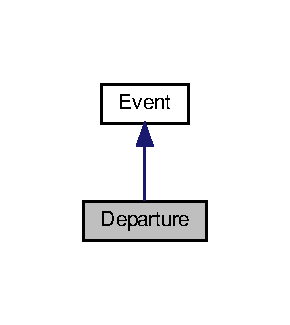
\includegraphics[width=139pt]{classDeparture__inherit__graph}
\end{center}
\end{figure}


Collaboration diagram for Departure\+:\nopagebreak
\begin{figure}[H]
\begin{center}
\leavevmode
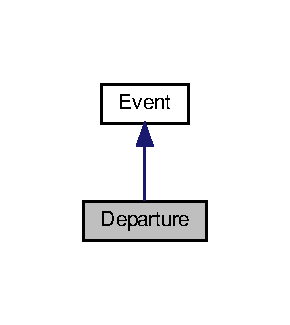
\includegraphics[width=139pt]{classDeparture__coll__graph}
\end{center}
\end{figure}
\subsection*{Public Member Functions}
\begin{DoxyCompactItemize}
\item 
\hyperlink{classDeparture_a6e0e7096d54c62c36110229266a8d37e}{Departure} (double time, \hyperlink{classClient}{Client} \&client, \hyperlink{classCashier}{Cashier} \&cashier)
\item 
\hyperlink{classDeparture_ade976c4ac1c737eded923e7e2adbf3f0}{Departure} (const \hyperlink{classDeparture}{Departure} \&departure)
\item 
void \hyperlink{classDeparture_a241611bdf4255d2ba868d58128dddc68}{process} () override
\end{DoxyCompactItemize}


\subsection{Detailed Description}
\hyperlink{classDeparture}{Departure} class, inheriting from \hyperlink{classEvent}{Event} class. Given private attributes are \+:
\begin{DoxyItemize}
\item cashier \hyperlink{classCashier}{Cashier} -\/ the cashier related to the \hyperlink{classDeparture}{Departure} event
\item client \hyperlink{classClient}{Client} -\/ the client who has just arrived in the bank 
\end{DoxyItemize}

\subsection{Constructor \& Destructor Documentation}
\mbox{\Hypertarget{classDeparture_a6e0e7096d54c62c36110229266a8d37e}\label{classDeparture_a6e0e7096d54c62c36110229266a8d37e}} 
\index{Departure@{Departure}!Departure@{Departure}}
\index{Departure@{Departure}!Departure@{Departure}}
\subsubsection{\texorpdfstring{Departure()}{Departure()}\hspace{0.1cm}{\footnotesize\ttfamily [1/2]}}
{\footnotesize\ttfamily Departure\+::\+Departure (\begin{DoxyParamCaption}\item[{double}]{time,  }\item[{\hyperlink{classClient}{Client} \&}]{client,  }\item[{\hyperlink{classCashier}{Cashier} \&}]{cashier }\end{DoxyParamCaption})}

\hyperlink{classDeparture}{Departure} Constructor 
\begin{DoxyParams}{Parameters}
{\em time} & Double -\/ the arrival time of the client \\
\hline
{\em client} & \hyperlink{classClient}{Client} -\/ the client who is leaving the bank \\
\hline
{\em cashier} & \hyperlink{classCashier}{Cashier} -\/ the cashier who served the client \\
\hline
\end{DoxyParams}
\mbox{\Hypertarget{classDeparture_ade976c4ac1c737eded923e7e2adbf3f0}\label{classDeparture_ade976c4ac1c737eded923e7e2adbf3f0}} 
\index{Departure@{Departure}!Departure@{Departure}}
\index{Departure@{Departure}!Departure@{Departure}}
\subsubsection{\texorpdfstring{Departure()}{Departure()}\hspace{0.1cm}{\footnotesize\ttfamily [2/2]}}
{\footnotesize\ttfamily Departure\+::\+Departure (\begin{DoxyParamCaption}\item[{const \hyperlink{classDeparture}{Departure} \&}]{departure }\end{DoxyParamCaption})}

\hyperlink{classDeparture}{Departure} Copy-\/\+Constructor 
\begin{DoxyParams}{Parameters}
{\em departure} & \hyperlink{classDeparture}{Departure} \\
\hline
\end{DoxyParams}


\subsection{Member Function Documentation}
\mbox{\Hypertarget{classDeparture_a241611bdf4255d2ba868d58128dddc68}\label{classDeparture_a241611bdf4255d2ba868d58128dddc68}} 
\index{Departure@{Departure}!process@{process}}
\index{process@{process}!Departure@{Departure}}
\subsubsection{\texorpdfstring{process()}{process()}}
{\footnotesize\ttfamily void Departure\+::process (\begin{DoxyParamCaption}{ }\end{DoxyParamCaption})\hspace{0.3cm}{\ttfamily [override]}, {\ttfamily [virtual]}}

Launch \hyperlink{classDeparture}{Departure}\textquotesingle{}s process. The cashier associated with the departure is going to be available, while the client will be destroyed. 

Implements \hyperlink{classEvent_af1940e82c4da67c8119f0dfe026949b4}{Event}.



The documentation for this class was generated from the following files\+:\begin{DoxyCompactItemize}
\item 
Departure.\+h\item 
Departure.\+cpp\end{DoxyCompactItemize}

\hypertarget{classDiscreteEventSimulation}{}\section{Discrete\+Event\+Simulation Class Reference}
\label{classDiscreteEventSimulation}\index{Discrete\+Event\+Simulation@{Discrete\+Event\+Simulation}}


Inheritance diagram for Discrete\+Event\+Simulation\+:
% FIG 0
\subsection*{Public Member Functions}
\begin{DoxyCompactItemize}
\item 
\hyperlink{classDiscreteEventSimulation_afef7ef964c3a7d151150120184c58d99}{Discrete\+Event\+Simulation} (double start\+Time)
\item 
\hyperlink{classDiscreteEventSimulation_aa92e10279fe95449f35139a4893192f5}{Discrete\+Event\+Simulation} (const \hyperlink{classDiscreteEventSimulation}{Discrete\+Event\+Simulation} \&discrete\+Event\+Simulation)
\item 
void \hyperlink{classDiscreteEventSimulation_a03770d2464931bc3555d4f34379aaa1e}{add\+Event} (\hyperlink{classEvent}{Event} $\ast$event)
\item 
double \hyperlink{classDiscreteEventSimulation_a41c5492fdf2d5ef2a9a27200871caabd}{get\+Current\+Time} ()
\item 
void \hyperlink{classDiscreteEventSimulation_aae616e227950798dc958171210975713}{launch} ()
\end{DoxyCompactItemize}


\subsection{Constructor \& Destructor Documentation}
\mbox{\Hypertarget{classDiscreteEventSimulation_afef7ef964c3a7d151150120184c58d99}\label{classDiscreteEventSimulation_afef7ef964c3a7d151150120184c58d99}} 
\index{Discrete\+Event\+Simulation@{Discrete\+Event\+Simulation}!Discrete\+Event\+Simulation@{Discrete\+Event\+Simulation}}
\index{Discrete\+Event\+Simulation@{Discrete\+Event\+Simulation}!Discrete\+Event\+Simulation@{Discrete\+Event\+Simulation}}
\subsubsection{\texorpdfstring{Discrete\+Event\+Simulation()}{DiscreteEventSimulation()}\hspace{0.1cm}{\footnotesize\ttfamily [1/2]}}
{\footnotesize\ttfamily Discrete\+Event\+Simulation\+::\+Discrete\+Event\+Simulation (\begin{DoxyParamCaption}\item[{double}]{start\+Time }\end{DoxyParamCaption})\hspace{0.3cm}{\ttfamily [explicit]}}

\hyperlink{classDiscreteEventSimulation}{Discrete\+Event\+Simulation} Constructor 
\begin{DoxyParams}{Parameters}
{\em start\+Time} & \\
\hline
\end{DoxyParams}
\mbox{\Hypertarget{classDiscreteEventSimulation_aa92e10279fe95449f35139a4893192f5}\label{classDiscreteEventSimulation_aa92e10279fe95449f35139a4893192f5}} 
\index{Discrete\+Event\+Simulation@{Discrete\+Event\+Simulation}!Discrete\+Event\+Simulation@{Discrete\+Event\+Simulation}}
\index{Discrete\+Event\+Simulation@{Discrete\+Event\+Simulation}!Discrete\+Event\+Simulation@{Discrete\+Event\+Simulation}}
\subsubsection{\texorpdfstring{Discrete\+Event\+Simulation()}{DiscreteEventSimulation()}\hspace{0.1cm}{\footnotesize\ttfamily [2/2]}}
{\footnotesize\ttfamily Discrete\+Event\+Simulation\+::\+Discrete\+Event\+Simulation (\begin{DoxyParamCaption}\item[{const \hyperlink{classDiscreteEventSimulation}{Discrete\+Event\+Simulation} \&}]{discrete\+Event\+Simulation }\end{DoxyParamCaption})}

\hyperlink{classDiscreteEventSimulation}{Discrete\+Event\+Simulation} Copy-\/\+Constructor 
\begin{DoxyParams}{Parameters}
{\em discrete\+Event\+Simulation} & \\
\hline
\end{DoxyParams}


\subsection{Member Function Documentation}
\mbox{\Hypertarget{classDiscreteEventSimulation_a03770d2464931bc3555d4f34379aaa1e}\label{classDiscreteEventSimulation_a03770d2464931bc3555d4f34379aaa1e}} 
\index{Discrete\+Event\+Simulation@{Discrete\+Event\+Simulation}!add\+Event@{add\+Event}}
\index{add\+Event@{add\+Event}!Discrete\+Event\+Simulation@{Discrete\+Event\+Simulation}}
\subsubsection{\texorpdfstring{add\+Event()}{addEvent()}}
{\footnotesize\ttfamily void Discrete\+Event\+Simulation\+::add\+Event (\begin{DoxyParamCaption}\item[{\hyperlink{classEvent}{Event} $\ast$}]{event }\end{DoxyParamCaption})}

Add the given event to event\+Queue 
\begin{DoxyParams}{Parameters}
{\em event} & \\
\hline
\end{DoxyParams}
\mbox{\Hypertarget{classDiscreteEventSimulation_a41c5492fdf2d5ef2a9a27200871caabd}\label{classDiscreteEventSimulation_a41c5492fdf2d5ef2a9a27200871caabd}} 
\index{Discrete\+Event\+Simulation@{Discrete\+Event\+Simulation}!get\+Current\+Time@{get\+Current\+Time}}
\index{get\+Current\+Time@{get\+Current\+Time}!Discrete\+Event\+Simulation@{Discrete\+Event\+Simulation}}
\subsubsection{\texorpdfstring{get\+Current\+Time()}{getCurrentTime()}}
{\footnotesize\ttfamily double Discrete\+Event\+Simulation\+::get\+Current\+Time (\begin{DoxyParamCaption}{ }\end{DoxyParamCaption})}

Get current time \begin{DoxyReturn}{Returns}
current\+Time 
\end{DoxyReturn}
\mbox{\Hypertarget{classDiscreteEventSimulation_aae616e227950798dc958171210975713}\label{classDiscreteEventSimulation_aae616e227950798dc958171210975713}} 
\index{Discrete\+Event\+Simulation@{Discrete\+Event\+Simulation}!launch@{launch}}
\index{launch@{launch}!Discrete\+Event\+Simulation@{Discrete\+Event\+Simulation}}
\subsubsection{\texorpdfstring{launch()}{launch()}}
{\footnotesize\ttfamily void Discrete\+Event\+Simulation\+::launch (\begin{DoxyParamCaption}{ }\end{DoxyParamCaption})}

Launch simulation 

The documentation for this class was generated from the following files\+:\begin{DoxyCompactItemize}
\item 
Discrete\+Event\+Simulation.\+h\item 
Discrete\+Event\+Simulation.\+cpp\end{DoxyCompactItemize}

\hypertarget{classEvent}{}\section{Event Class Reference}
\label{classEvent}\index{Event@{Event}}


{\ttfamily \#include $<$Event.\+h$>$}



Inheritance diagram for Event\+:\nopagebreak
\begin{figure}[H]
\begin{center}
\leavevmode
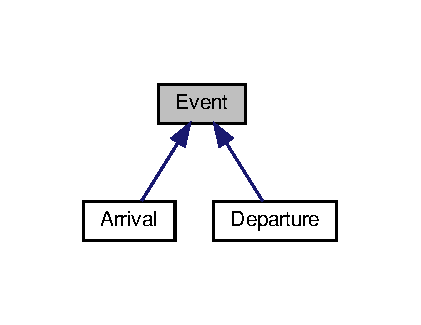
\includegraphics[width=202pt]{classEvent__inherit__graph}
\end{center}
\end{figure}
\subsection*{Public Member Functions}
\begin{DoxyCompactItemize}
\item 
\hyperlink{classEvent_aebd4c54256dbf46040053babdfcdf987}{Event} (double time)
\item 
\hyperlink{classEvent_ae8b35bf9237b74824194f87128e4fdab}{Event} (const \hyperlink{classEvent}{Event} \&event)
\item 
virtual void \hyperlink{classEvent_af1940e82c4da67c8119f0dfe026949b4}{process} ()=0
\item 
double \hyperlink{classEvent_ab05b23f7cc8d126efcbf189062f3b275}{get\+Time} ()
\end{DoxyCompactItemize}


\subsection{Detailed Description}
\hyperlink{classEvent}{Event} class, working as a virtual class. Given attribute is \+:
\begin{DoxyItemize}
\item time \+: double attribute indicating the time when the event took place 
\end{DoxyItemize}

\subsection{Constructor \& Destructor Documentation}
\mbox{\Hypertarget{classEvent_aebd4c54256dbf46040053babdfcdf987}\label{classEvent_aebd4c54256dbf46040053babdfcdf987}} 
\index{Event@{Event}!Event@{Event}}
\index{Event@{Event}!Event@{Event}}
\subsubsection{\texorpdfstring{Event()}{Event()}\hspace{0.1cm}{\footnotesize\ttfamily [1/2]}}
{\footnotesize\ttfamily Event\+::\+Event (\begin{DoxyParamCaption}\item[{double}]{time }\end{DoxyParamCaption})\hspace{0.3cm}{\ttfamily [explicit]}}

\hyperlink{classEvent}{Event} Constructor 
\begin{DoxyParams}{Parameters}
{\em time} & Double -\/ the arrival or departure time of the client \\
\hline
\end{DoxyParams}
\mbox{\Hypertarget{classEvent_ae8b35bf9237b74824194f87128e4fdab}\label{classEvent_ae8b35bf9237b74824194f87128e4fdab}} 
\index{Event@{Event}!Event@{Event}}
\index{Event@{Event}!Event@{Event}}
\subsubsection{\texorpdfstring{Event()}{Event()}\hspace{0.1cm}{\footnotesize\ttfamily [2/2]}}
{\footnotesize\ttfamily Event\+::\+Event (\begin{DoxyParamCaption}\item[{const \hyperlink{classEvent}{Event} \&}]{event }\end{DoxyParamCaption})}

\hyperlink{classEvent}{Event} Copy-\/\+Constructor 
\begin{DoxyParams}{Parameters}
{\em event} & \hyperlink{classEvent}{Event} \\
\hline
\end{DoxyParams}


\subsection{Member Function Documentation}
\mbox{\Hypertarget{classEvent_ab05b23f7cc8d126efcbf189062f3b275}\label{classEvent_ab05b23f7cc8d126efcbf189062f3b275}} 
\index{Event@{Event}!get\+Time@{get\+Time}}
\index{get\+Time@{get\+Time}!Event@{Event}}
\subsubsection{\texorpdfstring{get\+Time()}{getTime()}}
{\footnotesize\ttfamily double Event\+::get\+Time (\begin{DoxyParamCaption}{ }\end{DoxyParamCaption})}

Get time \begin{DoxyReturn}{Returns}
time Double 
\end{DoxyReturn}
\mbox{\Hypertarget{classEvent_af1940e82c4da67c8119f0dfe026949b4}\label{classEvent_af1940e82c4da67c8119f0dfe026949b4}} 
\index{Event@{Event}!process@{process}}
\index{process@{process}!Event@{Event}}
\subsubsection{\texorpdfstring{process()}{process()}}
{\footnotesize\ttfamily virtual void Event\+::process (\begin{DoxyParamCaption}{ }\end{DoxyParamCaption})\hspace{0.3cm}{\ttfamily [pure virtual]}}

Launch \hyperlink{classEvent}{Event}\textquotesingle{}s process 

Implemented in \hyperlink{classArrival_ad7da9fd4613164ece60d63be1bac6f1d}{Arrival}, and \hyperlink{classDeparture_a241611bdf4255d2ba868d58128dddc68}{Departure}.



The documentation for this class was generated from the following files\+:\begin{DoxyCompactItemize}
\item 
Event.\+h\item 
Event.\+cpp\end{DoxyCompactItemize}

\hypertarget{classPoisson}{}\section{Poisson Class Reference}
\label{classPoisson}\index{Poisson@{Poisson}}
\subsection*{Static Public Member Functions}
\begin{DoxyCompactItemize}
\item 
static void \hyperlink{classPoisson_ac616eec569fc0291dbd1cacf0f73108e}{init} (int seed=0)
\item 
static double \hyperlink{classPoisson_aaf4f6c620dba71a1e02fdb2a99f1f031}{next} (double moy=1.\+0)
\end{DoxyCompactItemize}


\subsection{Member Function Documentation}
\mbox{\Hypertarget{classPoisson_ac616eec569fc0291dbd1cacf0f73108e}\label{classPoisson_ac616eec569fc0291dbd1cacf0f73108e}} 
\index{Poisson@{Poisson}!init@{init}}
\index{init@{init}!Poisson@{Poisson}}
\subsubsection{\texorpdfstring{init()}{init()}}
{\footnotesize\ttfamily void Poisson\+::init (\begin{DoxyParamCaption}\item[{int}]{seed = {\ttfamily 0} }\end{DoxyParamCaption})\hspace{0.3cm}{\ttfamily [static]}}

Initialise \hyperlink{classPoisson}{Poisson}\textquotesingle{}s Law 
\begin{DoxyParams}{Parameters}
{\em seed} & \\
\hline
\end{DoxyParams}
\mbox{\Hypertarget{classPoisson_aaf4f6c620dba71a1e02fdb2a99f1f031}\label{classPoisson_aaf4f6c620dba71a1e02fdb2a99f1f031}} 
\index{Poisson@{Poisson}!next@{next}}
\index{next@{next}!Poisson@{Poisson}}
\subsubsection{\texorpdfstring{next()}{next()}}
{\footnotesize\ttfamily double Poisson\+::next (\begin{DoxyParamCaption}\item[{double}]{moy = {\ttfamily 1.0} }\end{DoxyParamCaption})\hspace{0.3cm}{\ttfamily [static]}}

Get a random following \hyperlink{classPoisson}{Poisson}\textquotesingle{}s Law 
\begin{DoxyParams}{Parameters}
{\em moy} & \\
\hline
\end{DoxyParams}
\begin{DoxyReturn}{Returns}
random 
\end{DoxyReturn}


The documentation for this class was generated from the following files\+:\begin{DoxyCompactItemize}
\item 
Poisson.\+h\item 
Poisson.\+cpp\end{DoxyCompactItemize}

\hypertarget{classQueue}{}\section{Queue Class Reference}
\label{classQueue}\index{Queue@{Queue}}


{\ttfamily \#include $<$Queue.\+h$>$}

\subsection*{Public Member Functions}
\begin{DoxyCompactItemize}
\item 
\hyperlink{classQueue_ae2647f6001471e160dc95362aba43313}{Queue} (\hyperlink{classBank}{Bank} \&bank)
\item 
\hyperlink{classQueue_a4d325dcdfe0550824d529b7aa11535b8}{Queue} (const \hyperlink{classQueue}{Queue} \&queue)
\item 
int \hyperlink{classQueue_ac52fd0970c24510a4d0d3086b027021a}{get\+Max\+Length} ()
\item 
double \hyperlink{classQueue_afc73e60fa330498b5efdbf267d4508c2}{get\+Average\+Length} ()
\item 
double \hyperlink{classQueue_a21c1c1c4732177f6b8d8433ae5b4d771}{get\+Average\+Waiting\+Time} ()
\item 
void \hyperlink{classQueue_aa4545b1d42237801b75e0f20c3cc0587}{add\+Client} (\hyperlink{classClient}{Client} \&client)
\item 
bool \hyperlink{classQueue_a65d9b23c23c917faa44981539bc34be7}{is\+Empty} ()
\item 
\hyperlink{classClient}{Client} $\ast$ \hyperlink{classQueue_a2767e32f2c7f51eedf0b75af9d944f67}{remove} ()
\end{DoxyCompactItemize}


\subsection{Detailed Description}
\hyperlink{classQueue}{Queue} class representing the queue of customers in the bank. Given private attributes are \+:
\begin{DoxyItemize}
\item client\+Queue \+: deque$<$\+Client $\ast$$>$ attribute, which is behaving as a F\+I\+FO (First In First out).
\item max\+Length \+: integer attribute, where the maximum length of the queue reached during the simulation is saved.
\item integral \+: double attribute where the result of the calculated integral is kept, used when calculating queue average length.
\item bank \+: Bank-\/\+Pointer attribute, for easy access to the bank instance.
\item waiting\+Time \+: double attribute, used when calculating average serving time. 
\end{DoxyItemize}

\subsection{Constructor \& Destructor Documentation}
\mbox{\Hypertarget{classQueue_ae2647f6001471e160dc95362aba43313}\label{classQueue_ae2647f6001471e160dc95362aba43313}} 
\index{Queue@{Queue}!Queue@{Queue}}
\index{Queue@{Queue}!Queue@{Queue}}
\subsubsection{\texorpdfstring{Queue()}{Queue()}\hspace{0.1cm}{\footnotesize\ttfamily [1/2]}}
{\footnotesize\ttfamily Queue\+::\+Queue (\begin{DoxyParamCaption}\item[{\hyperlink{classBank}{Bank} \&}]{bank }\end{DoxyParamCaption})\hspace{0.3cm}{\ttfamily [explicit]}}

\hyperlink{classQueue}{Queue} Constructor 
\begin{DoxyParams}{Parameters}
{\em bank} & Reference in which the queue is part of \\
\hline
\end{DoxyParams}
\mbox{\Hypertarget{classQueue_a4d325dcdfe0550824d529b7aa11535b8}\label{classQueue_a4d325dcdfe0550824d529b7aa11535b8}} 
\index{Queue@{Queue}!Queue@{Queue}}
\index{Queue@{Queue}!Queue@{Queue}}
\subsubsection{\texorpdfstring{Queue()}{Queue()}\hspace{0.1cm}{\footnotesize\ttfamily [2/2]}}
{\footnotesize\ttfamily Queue\+::\+Queue (\begin{DoxyParamCaption}\item[{const \hyperlink{classQueue}{Queue} \&}]{queue }\end{DoxyParamCaption})}

\hyperlink{classQueue}{Queue} Copy-\/\+Constructor 
\begin{DoxyParams}{Parameters}
{\em queue} & \\
\hline
\end{DoxyParams}


\subsection{Member Function Documentation}
\mbox{\Hypertarget{classQueue_aa4545b1d42237801b75e0f20c3cc0587}\label{classQueue_aa4545b1d42237801b75e0f20c3cc0587}} 
\index{Queue@{Queue}!add\+Client@{add\+Client}}
\index{add\+Client@{add\+Client}!Queue@{Queue}}
\subsubsection{\texorpdfstring{add\+Client()}{addClient()}}
{\footnotesize\ttfamily void Queue\+::add\+Client (\begin{DoxyParamCaption}\item[{\hyperlink{classClient}{Client} \&}]{client }\end{DoxyParamCaption})}

Add client to client\+Queue 
\begin{DoxyParams}{Parameters}
{\em client} & to be added in the queue. \\
\hline
\end{DoxyParams}
\mbox{\Hypertarget{classQueue_afc73e60fa330498b5efdbf267d4508c2}\label{classQueue_afc73e60fa330498b5efdbf267d4508c2}} 
\index{Queue@{Queue}!get\+Average\+Length@{get\+Average\+Length}}
\index{get\+Average\+Length@{get\+Average\+Length}!Queue@{Queue}}
\subsubsection{\texorpdfstring{get\+Average\+Length()}{getAverageLength()}}
{\footnotesize\ttfamily double Queue\+::get\+Average\+Length (\begin{DoxyParamCaption}{ }\end{DoxyParamCaption})}

Get average length of the queue during the simulation. \begin{DoxyReturn}{Returns}
average\+Length as a double value 
\end{DoxyReturn}
\mbox{\Hypertarget{classQueue_a21c1c1c4732177f6b8d8433ae5b4d771}\label{classQueue_a21c1c1c4732177f6b8d8433ae5b4d771}} 
\index{Queue@{Queue}!get\+Average\+Waiting\+Time@{get\+Average\+Waiting\+Time}}
\index{get\+Average\+Waiting\+Time@{get\+Average\+Waiting\+Time}!Queue@{Queue}}
\subsubsection{\texorpdfstring{get\+Average\+Waiting\+Time()}{getAverageWaitingTime()}}
{\footnotesize\ttfamily double Queue\+::get\+Average\+Waiting\+Time (\begin{DoxyParamCaption}{ }\end{DoxyParamCaption})}

Get average waiting time during the simulation. \begin{DoxyReturn}{Returns}
average\+Waiting\+Time as a double value. 
\end{DoxyReturn}
\mbox{\Hypertarget{classQueue_ac52fd0970c24510a4d0d3086b027021a}\label{classQueue_ac52fd0970c24510a4d0d3086b027021a}} 
\index{Queue@{Queue}!get\+Max\+Length@{get\+Max\+Length}}
\index{get\+Max\+Length@{get\+Max\+Length}!Queue@{Queue}}
\subsubsection{\texorpdfstring{get\+Max\+Length()}{getMaxLength()}}
{\footnotesize\ttfamily int Queue\+::get\+Max\+Length (\begin{DoxyParamCaption}{ }\end{DoxyParamCaption})}

Get max length of the queue reached during the simulation. \begin{DoxyReturn}{Returns}
max\+Length as an integer value 
\end{DoxyReturn}
\mbox{\Hypertarget{classQueue_a65d9b23c23c917faa44981539bc34be7}\label{classQueue_a65d9b23c23c917faa44981539bc34be7}} 
\index{Queue@{Queue}!is\+Empty@{is\+Empty}}
\index{is\+Empty@{is\+Empty}!Queue@{Queue}}
\subsubsection{\texorpdfstring{is\+Empty()}{isEmpty()}}
{\footnotesize\ttfamily bool Queue\+::is\+Empty (\begin{DoxyParamCaption}{ }\end{DoxyParamCaption})}

Get if client\+Queue is empty \begin{DoxyReturn}{Returns}

\begin{DoxyItemize}
\item true if client\+Queue is empty
\item Else return false 
\end{DoxyItemize}
\end{DoxyReturn}
\mbox{\Hypertarget{classQueue_a2767e32f2c7f51eedf0b75af9d944f67}\label{classQueue_a2767e32f2c7f51eedf0b75af9d944f67}} 
\index{Queue@{Queue}!remove@{remove}}
\index{remove@{remove}!Queue@{Queue}}
\subsubsection{\texorpdfstring{remove()}{remove()}}
{\footnotesize\ttfamily \hyperlink{classClient}{Client} $\ast$ Queue\+::remove (\begin{DoxyParamCaption}{ }\end{DoxyParamCaption})}

Remove first client from client\+Queue and returns it \begin{DoxyReturn}{Returns}
\hyperlink{classClient}{Client} 
\end{DoxyReturn}


The documentation for this class was generated from the following files\+:\begin{DoxyCompactItemize}
\item 
Queue.\+h\item 
Queue.\+cpp\end{DoxyCompactItemize}

\hypertarget{classSimulation}{}\section{Simulation Class Reference}
\label{classSimulation}\index{Simulation@{Simulation}}


Inheritance diagram for Simulation\+:
% FIG 0


Collaboration diagram for Simulation\+:
% FIG 1
\subsection*{Public Member Functions}
\begin{DoxyCompactItemize}
\item 
\hyperlink{classSimulation_a4709539e1e5ef724442ba1484d4a9ab8}{Simulation} (double planned\+Duration, double average\+Arrival\+Time, double $\ast$average\+Service\+Times, int cashiers\+Count)
\item 
\hyperlink{classSimulation_ad82aba6067f881a5c364ea6b6b317325}{Simulation} (const \hyperlink{classSimulation}{Simulation} \&simulation)
\item 
double \hyperlink{classSimulation_a242c58ccefca3705bdc47ee7827c24fe}{get\+Planned\+Duration} ()
\item 
double \hyperlink{classSimulation_a1e4f97c6011a0cbce91c5034c917ab46}{get\+Average\+Arrival\+Time} ()
\item 
\hyperlink{classBank}{Bank} \& \hyperlink{classSimulation_a280ef124f9f6395a446b36a9dd45e4bc}{get\+Bank} ()
\item 
void \hyperlink{classSimulation_af7d8147539e8ea62f83c44fa0431e27d}{set\+Real\+Duration} (double real\+Duration)
\item 
double \hyperlink{classSimulation_a18218154310af27c087def0936690346}{get\+Real\+Duration} ()
\end{DoxyCompactItemize}
\subsection*{Public Attributes}
\begin{DoxyCompactItemize}
\item 
\mbox{\Hypertarget{classSimulation_ae125e30e669048458632583d63c6683e}\label{classSimulation_ae125e30e669048458632583d63c6683e}} 
bool {\bfseries D\+E\+B\+UG} = false
\end{DoxyCompactItemize}


\subsection{Constructor \& Destructor Documentation}
\mbox{\Hypertarget{classSimulation_a4709539e1e5ef724442ba1484d4a9ab8}\label{classSimulation_a4709539e1e5ef724442ba1484d4a9ab8}} 
\index{Simulation@{Simulation}!Simulation@{Simulation}}
\index{Simulation@{Simulation}!Simulation@{Simulation}}
\subsubsection{\texorpdfstring{Simulation()}{Simulation()}\hspace{0.1cm}{\footnotesize\ttfamily [1/2]}}
{\footnotesize\ttfamily Simulation\+::\+Simulation (\begin{DoxyParamCaption}\item[{double}]{planned\+Duration,  }\item[{double}]{average\+Arrival\+Time,  }\item[{double $\ast$}]{average\+Service\+Times,  }\item[{int}]{cashiers\+Count }\end{DoxyParamCaption})}

\hyperlink{classSimulation}{Simulation} Constructor 
\begin{DoxyParams}{Parameters}
{\em planned\+Duration} & Planned Duration for the simulation \\
\hline
{\em average\+Arrival\+Time} & Average arrival time wanted for the simulation \\
\hline
{\em average\+Service\+Times} & Average service time wanted for the cashier \\
\hline
{\em cashiers\+Count} & Wanted number of cashiers for the bank \\
\hline
\end{DoxyParams}
\mbox{\Hypertarget{classSimulation_ad82aba6067f881a5c364ea6b6b317325}\label{classSimulation_ad82aba6067f881a5c364ea6b6b317325}} 
\index{Simulation@{Simulation}!Simulation@{Simulation}}
\index{Simulation@{Simulation}!Simulation@{Simulation}}
\subsubsection{\texorpdfstring{Simulation()}{Simulation()}\hspace{0.1cm}{\footnotesize\ttfamily [2/2]}}
{\footnotesize\ttfamily Simulation\+::\+Simulation (\begin{DoxyParamCaption}\item[{const \hyperlink{classSimulation}{Simulation} \&}]{simulation }\end{DoxyParamCaption})}

\hyperlink{classSimulation}{Simulation} Copy-\/\+Constructor 
\begin{DoxyParams}{Parameters}
{\em simulation} & \\
\hline
\end{DoxyParams}


\subsection{Member Function Documentation}
\mbox{\Hypertarget{classSimulation_a1e4f97c6011a0cbce91c5034c917ab46}\label{classSimulation_a1e4f97c6011a0cbce91c5034c917ab46}} 
\index{Simulation@{Simulation}!get\+Average\+Arrival\+Time@{get\+Average\+Arrival\+Time}}
\index{get\+Average\+Arrival\+Time@{get\+Average\+Arrival\+Time}!Simulation@{Simulation}}
\subsubsection{\texorpdfstring{get\+Average\+Arrival\+Time()}{getAverageArrivalTime()}}
{\footnotesize\ttfamily double Simulation\+::get\+Average\+Arrival\+Time (\begin{DoxyParamCaption}{ }\end{DoxyParamCaption})}

Get average arrival time. \begin{DoxyReturn}{Returns}
average\+Arrival\+Time as a double value 
\end{DoxyReturn}
\mbox{\Hypertarget{classSimulation_a280ef124f9f6395a446b36a9dd45e4bc}\label{classSimulation_a280ef124f9f6395a446b36a9dd45e4bc}} 
\index{Simulation@{Simulation}!get\+Bank@{get\+Bank}}
\index{get\+Bank@{get\+Bank}!Simulation@{Simulation}}
\subsubsection{\texorpdfstring{get\+Bank()}{getBank()}}
{\footnotesize\ttfamily \hyperlink{classBank}{Bank} \& Simulation\+::get\+Bank (\begin{DoxyParamCaption}{ }\end{DoxyParamCaption})}

Get bank. \begin{DoxyReturn}{Returns}
bank 
\end{DoxyReturn}
\mbox{\Hypertarget{classSimulation_a242c58ccefca3705bdc47ee7827c24fe}\label{classSimulation_a242c58ccefca3705bdc47ee7827c24fe}} 
\index{Simulation@{Simulation}!get\+Planned\+Duration@{get\+Planned\+Duration}}
\index{get\+Planned\+Duration@{get\+Planned\+Duration}!Simulation@{Simulation}}
\subsubsection{\texorpdfstring{get\+Planned\+Duration()}{getPlannedDuration()}}
{\footnotesize\ttfamily double Simulation\+::get\+Planned\+Duration (\begin{DoxyParamCaption}{ }\end{DoxyParamCaption})}

Get simulation\textquotesingle{}s planned duration. \begin{DoxyReturn}{Returns}
planned\+Duration as a double value 
\end{DoxyReturn}
\mbox{\Hypertarget{classSimulation_a18218154310af27c087def0936690346}\label{classSimulation_a18218154310af27c087def0936690346}} 
\index{Simulation@{Simulation}!get\+Real\+Duration@{get\+Real\+Duration}}
\index{get\+Real\+Duration@{get\+Real\+Duration}!Simulation@{Simulation}}
\subsubsection{\texorpdfstring{get\+Real\+Duration()}{getRealDuration()}}
{\footnotesize\ttfamily double Simulation\+::get\+Real\+Duration (\begin{DoxyParamCaption}{ }\end{DoxyParamCaption})}

Get simulation\textquotesingle{}s real duration \begin{DoxyReturn}{Returns}
real\+Duration 
\end{DoxyReturn}
\mbox{\Hypertarget{classSimulation_af7d8147539e8ea62f83c44fa0431e27d}\label{classSimulation_af7d8147539e8ea62f83c44fa0431e27d}} 
\index{Simulation@{Simulation}!set\+Real\+Duration@{set\+Real\+Duration}}
\index{set\+Real\+Duration@{set\+Real\+Duration}!Simulation@{Simulation}}
\subsubsection{\texorpdfstring{set\+Real\+Duration()}{setRealDuration()}}
{\footnotesize\ttfamily void Simulation\+::set\+Real\+Duration (\begin{DoxyParamCaption}\item[{double}]{real\+Duration }\end{DoxyParamCaption})}

Set simulation\textquotesingle{}s real duration 
\begin{DoxyParams}{Parameters}
{\em real\+Duration} & \\
\hline
\end{DoxyParams}


The documentation for this class was generated from the following files\+:\begin{DoxyCompactItemize}
\item 
Simulation.\+h\item 
Simulation.\+cpp\end{DoxyCompactItemize}

%--- End generated contents ---

% Index
\backmatter
\newpage
\phantomsection
\clearemptydoublepage
\addcontentsline{toc}{chapter}{Index}
\printindex

\end{document}
